\section{Appendix}
In this appendix, we first provide rigorous definitions of evaluation metrics (~\cref{sec:evaluation_metrics_supp}), then describe the data pre-processing step (~\cref{sec:datasets_supp}), network architectures (~\cref{sec:network_arch_supp}) and training on individual datasets (~\cref{sec:training_supp}) in more detail. We further provide additional results (~\cref{sec:additional_results_supp}), ablation studies (~\cref{sec:addtional_ablation_supp}) as well as a runtime analysis (~\cref{sec:timing}). Finally, we show more visualisations on \emph{3DLoMatch} and \emph{ModelLoNet} benchmarks (~\cref{sec:qualitative_supp}). 


\subsection{Evaluation Metrics}
\label{sec:evaluation_metrics_supp}
The evaluation metrics, which we use to assess model performance in Sec.~4 of the main paper and ~\cref{sec:additional_results_supp} of this appendix, are formally defined as follows:

\textbf{Inlier ratio} looks at the set of putative correspondences $(\mathbf{p}, \mathbf{q}) \in \mathcal{K}_{i j}$ found by reciprocal matching%
in feature space, and measures what fraction of them is "correct", in the sense that they lie within a threshold $\tau_1\!=\!10\,$cm after registering the two scans with the ground truth transformation $\overbar{T}_\mathbf{P}^ \mathbf{Q}$:
\begin{equation}
\mathrm{IR} = \frac{1}{\left|\mathcal{K}_{ij}\right|} \sum_{\left(\mathbf{p}, \mathbf{q}\right) \in \mathcal{K}_{ij}} \big[ ||\overbar{\mathbf{T}}_\mathbf{P}^ \mathbf{Q}(\mathbf{p})-\mathbf{q}||_2<\tau_{1} \big]  \;,
\end{equation}
with $[\cdot]$ the Iverson bracket.

\textbf{Feature Match recall} (FMR)~\cite{deng2018ppfnet} measures the fraction of point cloud pairs for which, based on the number of inlier correspondences, it is \emph{likely} that accurate transformation parameters can be recovered with a robust estimator such as RANSAC.
Note that FMR only checks whether the inlier ratio is above a threshold $\tau_2=0.05$. It does not test if the transformation can actually be determined from those correspondences, which in practice is not always the case, since their geometric configuration may be (nearly) degenerate, e.g., they might lie very close together or along a straight edge.
A single pair of point clouds counts as suitable for registration if%
\begin{equation}
    IR > \tau_2
\end{equation}

\textbf{Registration recall}~\cite{choi2015robust} is the most reliable metric, as it measures end-to-end performance on the actual task of point cloud registration. Specifically, it looks at the set of ground truth correspondences $\mathcal{H}_{i j}^{*}$ after applying the estimated transformation $T_\mathbf{P}^ \mathbf{Q}$, computes their root mean square error,
\begin{equation}
    \mathrm{RMSE} = \sqrt{\frac{1}{\left|\mathcal{H}_{i j}^{*}\right|} \sum_{\left(\mathbf{p}, \mathbf{q}\right) \in \mathcal{H}_{i j}^{*}}||\mathbf{T}_\mathbf{P}^ \mathbf{Q}(\mathbf{p}) -\mathbf{q}||_2^2}\;,
\end{equation}
and checks for what fraction of all point pairs $\mathrm{RMSE}\!<\!0.2$.
In keeping with the original evaluation script of \emph{3DMatch}, immediately adjacent point clouds are excluded, since they have very high overlap by construction.



\textbf{Chamfer distance} measures the quality of registration on synthetic data. We follow ~\cite{yew2020rpm} and use the \emph{modified} Chamfer distance metric:
\begin{equation}
\begin{aligned}
\tilde{C D}(\mathbf{P}, \mathbf{Q}) = & \frac{1}{|\mathbf{P}|} \sum\limits_{\mathbf{p} \in \mathbf{P}} \min\limits_{\mathbf{q} \in \mathbf{Q}_{\text{raw}}}\|\mathbf{T}_\mathbf{P}^ \mathbf{Q}(\mathbf{p})-\mathbf{q}\|_{2}^{2} + \\
& \frac{1}{|\mathbf{Q}|} \sum\limits_{\mathbf{q} \in \mathbf{Q}} \min\limits_{\mathbf{p} \in \mathbf{P}_{\text{raw}}}\|\mathbf{q}- \mathbf{T}_\mathbf{P}^ \mathbf{Q}(\mathbf{p})\|_{2}^{2}
\end{aligned}
\end{equation}
where $\mathbf{P}_{\text{raw}}\in \mathbb{R}^{2048\times3}$ and $\mathbf{Q}_{\text{raw}}\in \mathbb{R}^{2048\times3}$ are \emph{raw} source and target point clouds, $\mathbf{P} \in \mathbb{R}^{717\times3}$ and $\mathbf{Q} \in \mathbb{R}^{717\times3}$ are \emph{input} source and target point clouds. 

\textbf{Relative translation and rotation errors} (RTE/RRE) measures the deviations from the ground truth pose as: 
\begin{equation}
\begin{aligned}
\text{RTE} &= \|\mathbf{t} - \overbar{\mathbf{t}}\|_2\\
\text{RRE} &=\arccos\big(\frac{\mathrm{trace}{(\mathbf{R}^{T}\overbar{\mathbf{R}})-1}}{2}\big)
\end{aligned}
\end{equation}
where $\mathbf{R}$ and $\mathbf{t}$ denote the estimated rotation matrix and translation vector, respectively.

\textbf{Empirical Cumulative Distribution Function} (ECDF) measures the distribution of a set of values:
\begin{equation}
\begin{aligned}
\text{ECDF} (x) = \frac{\big|\{o_i < x\}\big|}{\big|O\big|}
\end{aligned}
\end{equation}
where $O$ is a set of values(ovelap ratios in our case) and $x \in [\min\{O\}, \max\{O\}]$.

\subsection{Dataset Preprocessing}
\label{sec:datasets_supp}
\paragraph{3DMatch}
\cite{zeng20163dmatch} is a collection of 62 scenes, combining earlier data from Analysis-by-Synthesis~\cite{valentin2016learning}, 7Scenes~\cite{shotton2013scene}, SUN3D~\cite{xiao2013sun3d}, RGB-D Scenes v.2~\cite{lai2014unsupervised}, and Halber~\etal~\cite{Halber2016StructuredGR}.  The official benchmark splits the data into 54 scenes for training and 8 for testing. Individual scenes are not only captured in different indoor spaces (e.g., bedrooms, offices, living rooms, restrooms) but also with different depth sensors (e.g., Microsoft Kinect, Structure Sensor, Asus Xtion Pro Live, and Intel RealSense). \emph{3DMatch} provides great diversity and allows our model to generalize across different indoor spaces. Individual scenes of \emph{3DMatch} are split into point cloud fragments, which are generated by fusing 50 consecutive depth frames using TSDF volumetric fusion~\cite{curless1996volumetric}. As a preprocessing step, we apply voxel-grid downsampling to all point clouds, and if multiple points fall into the same voxel, we randomly pick one.

\paragraph{ModelNet40}
For each CAD model of \emph{ModelNet40}, 2048 points are first generated by uniform sampling and scaled to fit into a unit sphere. Then we follow~\cite{yew2020rpm} to produce partial scans: for source partial point cloud, we uniformly sample a plane through the origin that splits the unit sphere into two half-spaces, shift that plane along its normal until $\lfloor 2048\cdot p_v \rfloor$ points are on one side, and discard the points on the other side; the target point cloud is generated in the same manner; then the two resulting, partial point clouds are randomly rotated, translated and jittered with Gaussian noise. For the rotation, we sample a random axis and a random angle \textless45$^\circ$. The translation is sampled in the range $[-0.5,0.5]$. Gaussian noise is applied per coordinate with $\sigma\!=\!0.05$. Finally, 717 points are randomly sampled from the $\lfloor 2048\cdot p_v \rfloor$ points.


\paragraph{odometryKITTI}
The dataset was captured using a Velodyne HDL-64 3D laser scanner by driving around the mid-size city of Karlsruhe, in rural areas and on highways. The ground truth poses are provided by GPS/IMU system. We follow ~\cite{bai2020d3feat} to use ICP to reduce the noise in the ground truth poses. 


\subsection{Implementation and Training}
\begin{table}[t]
    \setlength{\tabcolsep}{6pt}
    \renewcommand{\arraystretch}{1.2}
	\centering
	\resizebox{\columnwidth}{!}{
    \begin{tabular}{cccccccc}
			\toprule
             & $n_p$ & $\gamma$ & $V$ & $r_p$ & $r_s$ & $r_o$ & $r_m$\\
            \hline
            \multicolumn{1}{c}{\emph{3DMatch}} & 256 & 24 & 0.025 & 0.0375 & 0.1 & 0.0375 & 0.05\\
            \multicolumn{1}{c}{\emph{ModelNet}} & 384 & 64 & 0.06 & 0.018 & 0.06 & 0.04 & 0.04 \\
            \multicolumn{1}{c}{\emph{odometryKITTI}} & 512 & 48 & 0.3 & 0.21 & 0.75 & 0.45 & 0.3 \\
			\bottomrule
			
	\end{tabular}
	}
	\caption{Hyper-parameters configurations for different datasets.}
	\label{tab:hyperparameters}
	
\end{table}
\label{sec:training_supp}
For 3DMatch/Modelnet/KITTI, we train \acro\ using Stochastic Gradient Descent for $30$/ $200$/ $150$ epochs, with initial learning rate $0.005$/ $0.01$/ $0.05$, momentum $0.98$, and weight decay $10^{-6}$. The learning rate is exponentially decayed by 0.05 after each epoch. Due to memory constraints we use batch size $1$ in all experiments. The dataset-dependent hyper-parameters which include number of negative pairs in circle loss $n_p$, temperature factor $\gamma$, voxel size $V$, search radius for positive pair $r_p$, safe radius $r_s$, overlap and matchability radius $r_o$ and $r_m$ are given in Tab.~\ref{tab:hyperparameters}. On odometryKITTI dataset, we take the curriculum learning~\cite{bengio2009curriculum} strategy to gradually learn sharper local descriptors by adjusting $n_p$. For more details please see our code.

\subsection{Network Architecture}
\label{sec:network_arch_supp}
% \begin{table}[t]
%     \setlength{\tabcolsep}{6pt}
%     \renewcommand{\arraystretch}{1.2}
% 	\centering
% 	\resizebox{0.7\columnwidth}{!}{
%     \begin{tabular}{ccccc}
% 			\toprule
%             \multicolumn{1}{c}{} & \multicolumn{1}{c}{\# strided} & \multicolumn{1}{c}{convolution} & \multicolumn{1}{c}{first conv.} & \multicolumn{1}{c}{final}\\
%             \multicolumn{1}{c}{} & \multicolumn{1}{c}{convolutions} & \multicolumn{1}{c}{radius} & \multicolumn{1}{c}{feature dim.} & \multicolumn{1}{c}{feature dim.}\\
%             \hline
%             \multicolumn{1}{c}{\emph{3DMatch}} & 3 & 2.5 & 64 & 32 \\
%             \multicolumn{1}{c}{\emph{ModelNet}} & 2 & 2.75 & 256 & 96 \\
%             \multicolumn{1}{c}{\emph{odometryKITTI}} & 3 & 4.25 & 128 & 32 \\
% 			\bottomrule
% 	\end{tabular}}
% 	\caption{Different network configurations for \emph{3DMatch}, \emph{ModelNet} and \emph{odometryKITTI} datasets.}
% 	\label{tab:compare_network}
% \end{table}

\begin{table}[t]
    \setlength{\tabcolsep}{6pt}
    \renewcommand{\arraystretch}{1.2}
	\centering
    \begin{tabularx}{\textwidth}{lYYYYY|YYYYY}
			\toprule
			& \multicolumn{5}{c|}{\textit{3DMatch}} & \multicolumn{5}{c}{\textit{3DLoMatch}} \\
			\# Samples & 5000 & 2500 & 1000 & 500 & 250 & 5000 & 2500 & 1000 & 500 & 250 \\
            \midrule
			& \multicolumn{10}{c}{\textit{Registration Recall (\%)}} \\
		    \midrule
 			3DSN~\cite{gojcic20193DSmoothNet} & 78.4 & 76.2 & 71.4 & 67.6 & 50.8 & 33.0 & 29.0 & 23.3 & 17.0 & 11.0  \\
 			FCGF~\cite{Choy2019FCGF} & \underline{85.1} & \underline{84.7} & 83.3 & 81.6 & 71.4 & \underline{40.1} & 41.7 & 38.2 & 35.4 & 26.8 \\
 			D3Feat~\cite{bai2020d3feat} & 81.6 & 84.5 & \underline{83.4} & \underline{82.4} & \underline{77.9} & 37.2 & \underline{42.7} & \underline{46.9} & \underline{43.8} & \underline{39.1} \\
 			\acro\ & \textbf{89.0} & \textbf{89.9} & \textbf{90.6} & \textbf{88.5} & \textbf{86.6} & \textbf{59.8} & \textbf{61.2} & \textbf{62.4} & \textbf{60.8} & \textbf{58.1} \\
			\bottomrule
	\end{tabularx}
	\caption{Results on the \emph{3DMatch} and \emph{3DLoMatch} datasets.}
	\label{tab:big_predator}
    
\end{table}
The detailed network architecture of \acro\ is depicted in Fig.~\ref{fig:network_arch_detailed}. Our model is built on the KPConv implementation from the D3Feat repository.%
\footnote{\url{https://github.com/XuyangBai/D3Feat.pytorch}} %
We complement each KPConv layer with instance normalisation Leaky ReLU activations. The $l$-th strided convolution is applied to a point cloud dowsampled with voxel size $2^{l}\cdot V$. Upsampling in the decoder is performed by querying the associated feature of the closest point from the previous layer.  

With $\approx$20k points after voxel-grid downsampling, the point clouds in \emph{3DMatch}  are much denser than those of \emph{ModelNet40} with only 717 points. Moreover, they also have larger spatial extent with bounding boxes up to $3\times3\times3$~$\text{m}^3$, while \emph{ModelNet40} point clouds are normalised to fit into a unit sphere.
To account for these large differences, we slightly adapt the encoder and decoder per dataset, but keep the same overlap attention model. Differences in network hyper-parameters are shown in Tab.~\ref{tab:compare_network}. 


\begin{table}[t!]
    \setlength{\tabcolsep}{6pt}
    \renewcommand{\arraystretch}{1.2}
	\centering
	\resizebox{\columnwidth}{!}{
    \begin{tabular}{lcccccccccc|cccccccccc}
			\toprule
			& \multicolumn{10}{c|}{\textit{3DMatch}} & \multicolumn{10}{c}{\textit{3DLoMatch}} \\
			& Kitchen & Home 1 & Home 2 & Hotel 1 & Hotel 2 & Hotel 3 & Study & MIT Lab & Avg. & STD	& Kitchen & Home 1 & Home 2 & Hotel 1 & Hotel 2 & Hotel 3 & Study & MIT Lab & Avg. & STD\\
            \midrule
            & \multicolumn{20}{c}{\textit{\# Sample}} \\
            \midrule
            & \textbf{449} & 106 & 159 & 182 & 78 & 26 & \underline{234} & 45 & 160 & 128 & \textbf{524} & \underline{283} & 222 & 210 & 138 & 42 & 237 & 70 & 191 & 154\\
			\midrule
			& \multicolumn{20}{c}{\textit{Registration Recall (\%)}~$\uparrow$} \\
			\midrule
			3DSN~\cite{gojcic20193DSmoothNet} & 90.6 & 90.6 & 65.4 & 89.6 & 82.1 & 80.8 & 68.4 & 60.0 & 78.4 & 11.5 & 51.4 & 25.9 & 44.1 & 41.1 & 30.7 & 36.6 & 14.0 & 20.3 & 33.0 & 11.8 \\
			FCGF~\cite{Choy2019FCGF} & \textbf{98.0} & \underline{94.3} & \underline{68.6} & \textbf{96.7} & \underline{91.0} & \textbf{84.6} & 76.1 & \underline{71.1} & \underline{85.1} & 11.0 & \underline{60.8} & \underline{42.2} & \underline{53.6} & \underline{53.1} & \underline{38.0} & 26.8 & \underline{16.1} & 30.4 & \underline{40.1} & 14.3\\
			D3Feat~\cite{bai2020d3feat} & 96.0 & 86.8 & 67.3 & 90.7 & 88.5 & 80.8 & \underline{78.2} & 64.4 & 81.6 & \underline{10.5} & 49.7 & 37.2 & 47.3 & 47.8 & 36.5 & \underline{31.7} & 15.7 & \underline{31.9} & 37.2 & \textbf{10.6}\\
			Ours & \underline{97.6} & \textbf{97.2} & \textbf{74.8} & \textbf{98.9} & \textbf{96.2} & \textbf{88.5} & \textbf{85.9} & \textbf{73.3} & \textbf{89.0} & \textbf{9.6} & \textbf
			{71.5} & \textbf{58.2} & \textbf{60.8} & \textbf{77.5} & \textbf{64.2} & \textbf{61.0} & \textbf{45.8} & \textbf{39.1} & \textbf{59.8} & \underline{11.7} \\
			\midrule
			& \multicolumn{20}{c}{\textit{Relative Rotation Error (\degree)}~$\downarrow$} \\
			\midrule
			3DSN~\cite{gojcic20193DSmoothNet} & 1.926 & 1.843 & \underline{2.324} & 2.041 & 1.952 & 2.908 & 2.296 & 2.301 & 2.199 & 0.321 & \underline{3.020} & 3.898 & 3.427 & 3.196 & 3.217 & 3.328 & 4.325 & 3.814 & 3.528 & 0.414\\
			FCGF~\cite{Choy2019FCGF} & \textbf{1.767} & \underline{1.849} & \textbf{2.210} & \textbf{1.867} & \underline{1.667} & \underline{2.417} & \textbf{2.024} & \textbf{1.792} & \textbf{1.949} & \underline{0.236} & \textbf{2.904} & \underline{3.229} & \underline{3.277} & \underline{2.768} & \textbf{2.801} & \textbf{2.822} & \underline{3.372} & 4.006 & \underline{3.147} & 0.394\\
			D3Feat~\cite{bai2020d3feat} & 2.016 & 2.029 & 2.425 & \underline{1.990} & 1.967 & \textbf{2.400} & 2.346 & 2.115 & 2.161 & \textbf{0.183} & 3.226 & 3.492 & 3.373 & 3.330 & 3.165 & \underline{2.972} & 3.708 & \underline{3.619} & 3.361 & \textbf{0.227} \\
			Ours & \underline{1.861} & \textbf{1.806} & 2.473 & 2.045 & \textbf{1.600} & 2.458 & \underline{2.067} & \underline{1.926} & \underline{2.029} & 0.286 & 3.079 & \textbf{2.637} & \textbf{3.220} & \textbf{2.694} & \underline{2.907} & 3.390 & \textbf{3.046} & \textbf{3.412} & \textbf{3.048} & \underline{0.273}\\
			\midrule
			& \multicolumn{20}{c}{\textit{Relative Translation Error (m)}~$\downarrow$} \\
			\midrule
			3DSN~\cite{gojcic20193DSmoothNet} & 0.059 & 0.070 & 0.079 & 0.065 & 0.074 & 0.062 & 0.093 & 0.065 & 0.071 & \textbf{0.010} & \underline{0.082} & 0.098 & 0.096 & 0.101 & \textbf{0.080} & 0.089 & 0.158 & \textbf{0.120} & 0.103 & 0.024\\
			FCGF~\cite{Choy2019FCGF} & \underline{0.053} & \underline{0.056} & \underline{0.071} & \textbf{0.062} & \underline{0.061} & \underline{0.055} & \underline{0.082} & 0.090 & \underline{0.066} & 0.013 & 0.084 & \underline{0.097} & \textbf{0.076} & 0.101 & \underline{0.084} & \underline{0.077} & \underline{0.144} & 0.140 & \underline{0.100} & 0.025\\
			D3Feat~\cite{bai2020d3feat} & 0.055 & 0.065 & 0.080 & \underline{0.064} & 0.078 & \textbf{0.049} & 0.083 & \underline{0.064} & 0.067 & 0.011 & 0.088 & 0.101 & 0.086 & \underline{0.099} & 0.092 & \textbf{0.075} & 0.146 & 0.135 & 0.103 & \underline{0.023}\\
			Ours & \textbf{0.048} & \textbf{0.055} & \textbf{0.070} & 0.073 & \textbf{0.060} & 0.065 & \textbf{0.080} & \textbf{0.063} & \textbf{0.064} & \underline{0.010} & \textbf{0.081} & \textbf{0.080} & \underline{0.084} & \textbf{0.099} & 0.096 & 0.077 & \textbf{0.101} & \underline{0.130} & \textbf{0.093} & \textbf{0.016}\\
			\bottomrule
	\end{tabular}
	}
	\caption{Detailed results on the \emph{3DMatch} and \emph{3DLoMatch} datasets.}
	\label{tab:detailed_3dmatch}
\end{table}


\subsection{Additional Results}
\label{sec:additional_results_supp}
\paragraph{Detailed registration results}
We report detailed per-scene \textit{Registration Recall (RR)}, \textit{Relative Rotation Error (RRE)} and \textit{Relative Translation Error (RTE)} in Tab.~\ref{tab:detailed_3dmatch}. RRE and RTE are only averaged over successfully registered pairs for each scene, such that the numbers are mot dominated by gross errors from complete registration failures. We get the highest RR and lowest or second lowest RTE and RRE for almost all scenes, this further shows that our overlap attention module together with probabilistic sampling supports not only robust, but also accurate registration.  


\paragraph{Feature match recall}
Finally, Fig.~\ref{fig:fmr} shows that our descriptors are robust and perform well over a wide range of thresholds for the allowable inlier distance and the minimum inlier ratio. Notably, \acro\ consistently outperforms D3Feat that uses a similar KPConv backbone.


\subsection{Additional Ablation Studies}
\label{sec:addtional_ablation_supp}

\begin{table}[t!]
    \setlength{\tabcolsep}{6pt}
    \renewcommand{\arraystretch}{1.2}
	\centering
	\resizebox{\columnwidth}{!}{
    \begin{tabular}{ll|cccccc}
			\toprule
			\multicolumn{2}{c}{} & \multicolumn{3}{c}{\textit{3DMatch}} & \multicolumn{3}{c}{\textit{3DLoMatch}} \\
            \cline{3-8}
            \scalebox{.8}[1.0]{matchability} & \multicolumn{1}{c}{\scalebox{.8}[1.0]{overlap}} & FMR & IR & RR & FMR & IR & RR \\
            \hline
            \multicolumn{1}{c}{} & \multicolumn{1}{c}{} & \underline{96.2} & 51.6 & 86.0 & 74.9 & 20.4 & 43.3 \\
            \multicolumn{1}{c}{\ding{51}} & \multicolumn{1}{c}{} & 96.1 & 54.0 & \textbf{89.2} & 75.5 & 21.9 & 52.2 \\
            \multicolumn{1}{c}{} & \multicolumn{1}{c}{\ding{51}} & \underline{96.2} & \underline{56.7} & \underline{89.1} & \underline{78.3} & \underline{26.1} & \underline{57.4}\\
            \multicolumn{1}{c}{\ding{51}} & \multicolumn{1}{c}{\ding{51}} & \textbf{96.7} & \textbf{58.0} & 89.0 & \textbf{78.6} & \textbf{26.7} & \textbf{59.8}\\
			\bottomrule
	\end{tabular}
	}
	\caption{Different combinations of scores used for probabilistic sampling.}
	\label{tab:ablate_matchability}
\end{table}
\paragraph{Ablations of matchability score}
We find that probabilistic sampling guided by the product of the overlap and matchability scores attains the highest RR. Here we further analyse the impact of each individual component. We first construct a baseline which applies random sampling (\textit{rand}) over conditioned features, then we sample points with probability proportional to overlap scores (\textit{prob. (o)}), to matchability scores (\textit{prob. (m)}), and to the combination of the two scores (\textit{prob. (om)}). As shown in Tab.~\ref{tab:ablate_matchability}, \textit{rand} fares clearly worse, in all metrics. Compared to \textit{prob. (om)}, either \textit{prob. (o)} or \textit{prob. (m)} can achieve comparable results on \emph{3DMatch}; the performance gap becomes big on the more challenging \emph{3DLoMatch} dataset, where our \textit{prob. (om)} is around 4 pp better in terms of RR. 

% \begin{table}[t]
%     \setlength{\tabcolsep}{6pt}
%     \renewcommand{\arraystretch}{1.2}
% 	\centering
% 	\resizebox{0.9\columnwidth}{!}{
%     \begin{tabular}{lccccc|ccccc}
% 			\toprule
% 			& \multicolumn{5}{c|}{\textit{3DMatch}} & \multicolumn{5}{c}{\textit{3DLoMatch}} \\
% 			\# Samples & 5000 & 2500 & 1000 & 500 & 250 & 5000 & 2500 & 1000 & 500 & 250 \\
%             \midrule
% 			& \multicolumn{10}{c}{\textit{Registration Recall (\%)}} \\
% 		    \midrule
%  			FCGF~\cite{Choy2019FCGF} & 85.1 & 84.7 & 83.3 & 81.6 & 71.4 & 40.1 & 41.7 & 38.2 & 35.4 & 26.8 \\
%  			FCGF+OA& \textbf{89.1} & \textbf{88.9} & \textbf{88.7} & \textbf{87.5} & \textbf{85.4} & \textbf{57.8} & \textbf{58.3} & \textbf{59.8} & \textbf{58.7} & \textbf{55.9}\\
% 			\bottomrule
			
% 	\end{tabular}
% 	}
% 	\caption{Ablation of the proposed overlap attention module with sparse convolution backbone. FCGF + OA denotes adding proposed overlap attention module to FCGF model.}
% 	\label{tab:ablate_fcgf}
% \end{table}


\begin{table}[t]
    \setlength{\tabcolsep}{6pt}
    \renewcommand{\arraystretch}{1.2}
	\centering
    \begin{tabularx}{\columnwidth}{lYYYYY|YYYYY}
			\toprule
			& \multicolumn{5}{c|}{\textit{3DMatch}} & \multicolumn{5}{c}{\textit{3DLoMatch}} \\
			\# Samples & 5000 & 2500 & 1000 & 500 & 250 & 5000 & 2500 & 1000 & 500 & 250 \\
            \midrule
			& \multicolumn{10}{c}{\textit{Registration Recall (\%)}} \\
		    \midrule
 			FCGF~\cite{Choy2019FCGF} & 85.1 & 84.7 & 83.3 & 81.6 & 71.4 & 40.1 & 41.7 & 38.2 & 35.4 & 26.8 \\
 			FCGF+OA& \textbf{89.1} & \textbf{88.9} & \textbf{88.7} & \textbf{87.5} & \textbf{85.4} & \textbf{57.8} & \textbf{58.3} & \textbf{59.8} & \textbf{58.7} & \textbf{55.9}\\
			\bottomrule
			
	\end{tabularx}
	\caption{Ablation of the proposed overlap attention module with sparse convolution backbone. FCGF + OA denotes adding proposed overlap attention module to FCGF model.}
	\label{tab:ablate_fcgf}
\end{table}
\paragraph{Ablations of overlap attention module with FCGF}
To demonstrate the flexibility of our model, we additionally add proposed overlap attention module to FCGF model. We train it on \emph{3DMatch} dataset with our proposed loss for 100 epochs, the results are shown in Tab.~\ref{tab:ablate_fcgf}. It shows that FCGF can also greatly benefit from the overlap attention module. Registration recall almost doubles when sampling only 250 points on the challenging \emph{3DLoMatch} benchmark. 

\begin{figure}[t!]
    \centering
    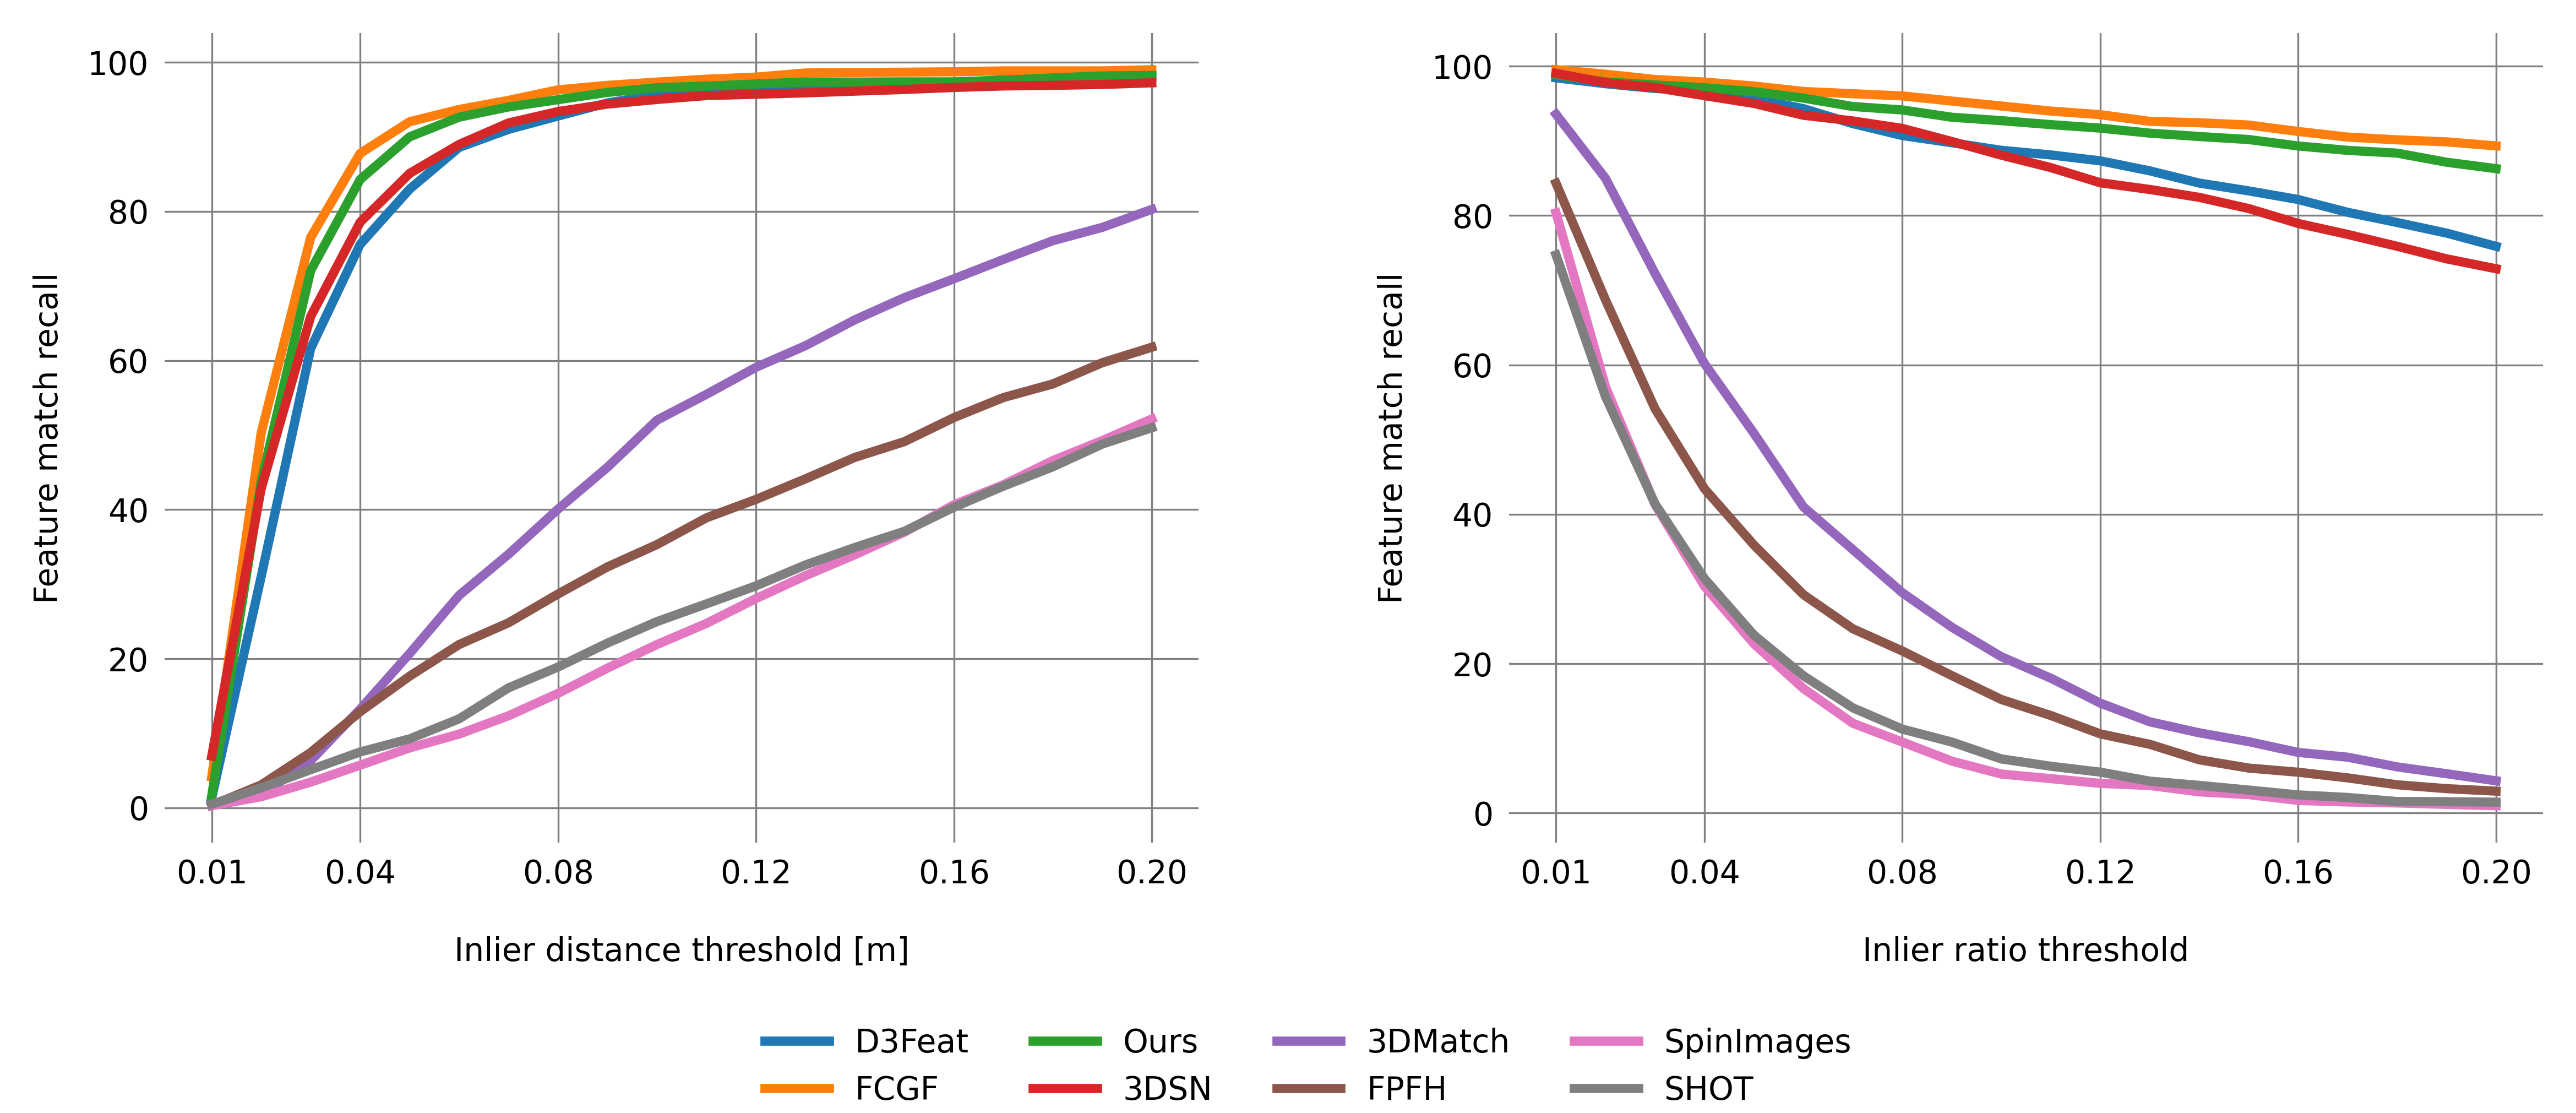
\includegraphics[width=\columnwidth]{figures/images/fmr.png}

    \caption{Feature matching recall in relation to inlier distance threshold $\tau_{1}$ (left) and inlier ratio threshold $\tau_{2}$ (right)}
    \label{fig:fmr}
\end{figure}
\subsection{Timings}
\label{sec:timing}
% \begin{table}[t!]
%     \setlength{\tabcolsep}{6pt}
%     \renewcommand{\arraystretch}{1.2}
% 	\centering
% 	\resizebox{\columnwidth}{!}{
%     \begin{tabular}{ccccccc}
% 			\toprule
%             \multicolumn{2}{c}{} & \multicolumn{1}{c}{\renewcommand{\arraystretch}{0.8}\begin{tabular}{c}\scalebox{0.9}[1.0]{data}\\\scalebox{0.9}[1.0]{loader}\end{tabular}} & \multicolumn{1}{c}{\scalebox{0.9}[1.0]{encoder}} & \multicolumn{1}{c}{\renewcommand{\arraystretch}{0.8}\begin{tabular}{c}\scalebox{0.9}[1.0]{overlap}\\\scalebox{0.9}[1.0]{attention}\end{tabular}} & \multicolumn{1}{c}{\scalebox{0.9}[1.0]{decoder}} &
%             \multicolumn{1}{c}{\scalebox{0.9}[1.0]{overall}} \\
%             \hline
%             \multicolumn{2}{c}{FCGF~\cite{Choy2019FCGF}} & \textcolor{white}{20}\textbf{6} & 414 & --- & 25 & 445 \\
%             \multicolumn{2}{c}{D3Feat~\cite{bai2020d3feat}} & 200 & \textcolor{white}{4}\underline{11} & --- & \underline{63} & \underline{274}\\
%             \multicolumn{2}{c}{Ours} & \underline{191} & \textcolor{white}{41}\textbf{9} & 70 & \textcolor{white}{6}\textbf{1} & \textbf{271}\\ 
% 			\bottomrule
% 	\end{tabular}}
% 	\caption{Runtime per fragment pair in milli-seconds, averaged over 1623 test pairs of \emph{3DMatch}.}
% 	\label{tab:3DMatch_times}
% \end{table}

\begin{table}[t]
    \setlength{\tabcolsep}{2pt}
    \renewcommand{\arraystretch}{1.2}
	\centering
    \begin{tabularx}{\textwidth}{lYYYYY}
			\toprule
            \multicolumn{1}{c}{} & \multicolumn{1}{c}{\renewcommand{\arraystretch}{0.8}\begin{tabular}{c}\scalebox{0.9}[1.0]{data}\\\scalebox{0.9}[1.0]{loader}\end{tabular}} & \multicolumn{1}{c}{\scalebox{0.9}[1.0]{encoder}} & \multicolumn{1}{c}{\renewcommand{\arraystretch}{0.8}\begin{tabular}{c}\scalebox{0.9}[1.0]{overlap}\\\scalebox{0.9}[1.0]{attention}\end{tabular}} & \multicolumn{1}{c}{\scalebox{0.9}[1.0]{decoder}} &
            \multicolumn{1}{c}{\scalebox{0.9}[1.0]{overall}} \\
            \hline
            FCGF~\cite{Choy2019FCGF} & \textbf{6} & 414 & --- & 25 & 445 \\
            D3Feat~\cite{bai2020d3feat} & 200 & \underline{11} & --- & \underline{63} & \underline{274}\\
            Ours & \underline{191} & \textbf{9} & 70 & \textbf{1} & \textbf{271}\\ 
			\bottomrule
	\end{tabularx}
	\caption{Runtime per fragment pair in milli-seconds, averaged over 1623 test pairs of \emph{3DMatch}.}
	\label{tab:3DMatch_times}
\end{table}
We compare the runtime of \acro\ with FCGF%
\footnote{All experiments were done with MinkowskiEngine v0.4.2.} %
~\cite{Choy2019FCGF} and D3Feat%
\footnote{We use its PyTorch implementation.} %
~\cite{bai2020d3feat} on \emph{3DMatch}. For all three methods we set voxel size $V\!=\!2.5\,$cm and batch size 1. The test is run on a single GeForce GTX 1080 Ti with Intel(R) Core(TM) i7-7700K CPU @ 4.20GHz, 32GB RAM. The most time-consuming step of our model, and also of D3Feat, is the data loader, as we have to pre-compute the neighborhood indices before the forward pass. With its smaller encoder and decoder, but the additional overlap attention module, \acro\ is still marginally faster than D3Feat. FCGF has a more efficient data loader that relies on sparse convolution and queries neighbors during the forward pass. See Tab.~\ref{tab:3DMatch_times}.

\subsection{Qualitative Visualization}
\label{sec:qualitative_supp}
We show more qualitative results in Fig.~\ref{fig:3dmatch_supp} and Fig.~\ref{fig:modelnet_supp} for \emph{3DLoMatch} and \emph{ModelLoNet} respectively. The input points clouds are rotated and translated here for better visualization of overlap and matchability scores. 

\begin{figure}[t]
    \centering
    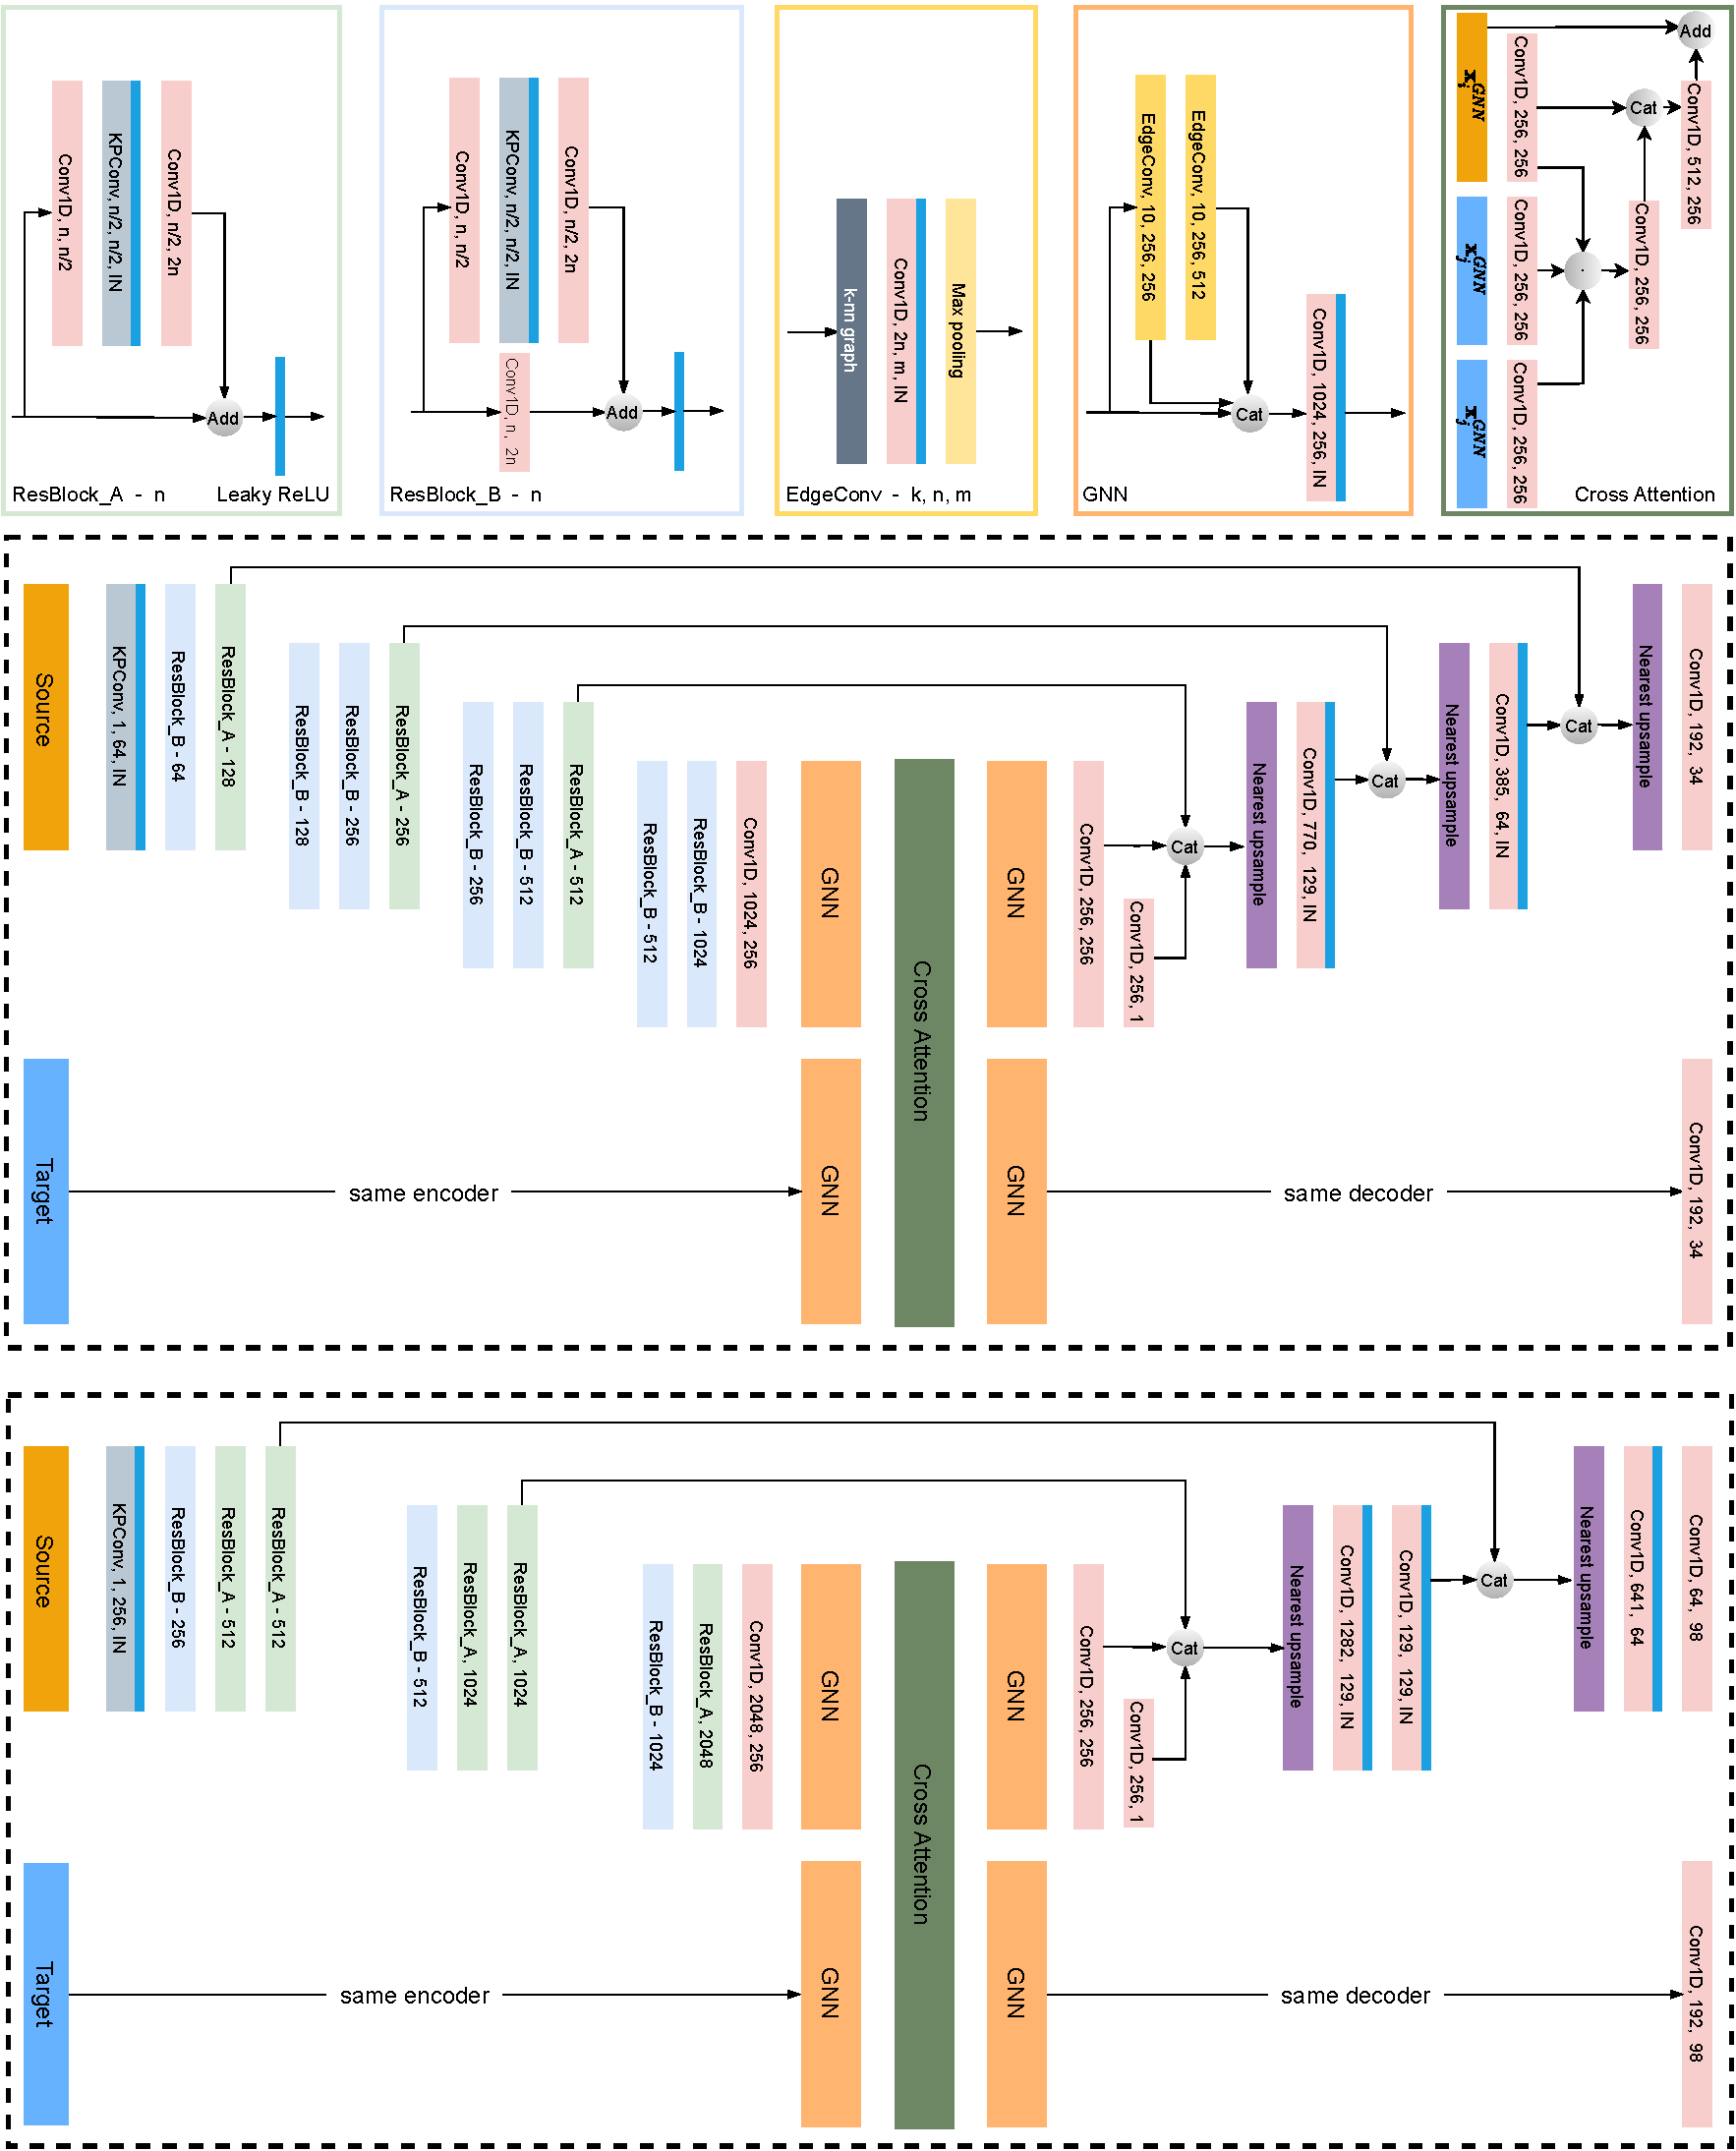
\includegraphics[width=1.0\columnwidth]{figures/images/arch_sketch.pdf}
    \caption{Network architecture of \acro\ for \emph{3DMatch} (\textit{middle}) and \emph{ModelNet} (\textit{bottom}). In the cross attention module, for each (query $\mathbf{s}_i \in \mathbb{R}^{b\times1}$ , key $\mathbf{k}_i \in \mathbb{R}^{b\times1}$, value $\mathbf{v}_i \in \mathbb{R}^{b\times1}$), $\bigodot$ denotes first reshape them into shape $(4, \frac{b}{4})$(4 heads), then compute scores matrix $\mathbf{S}$ from $\mathbf{s}_i$ and $\mathbf{k}_i$, finally get message update from $\mathbf{v}_i$ and reshape back to $(b,1)$.}
    \label{fig:network_arch_detailed}
\end{figure}
\begin{figure}[t]
    \centering
    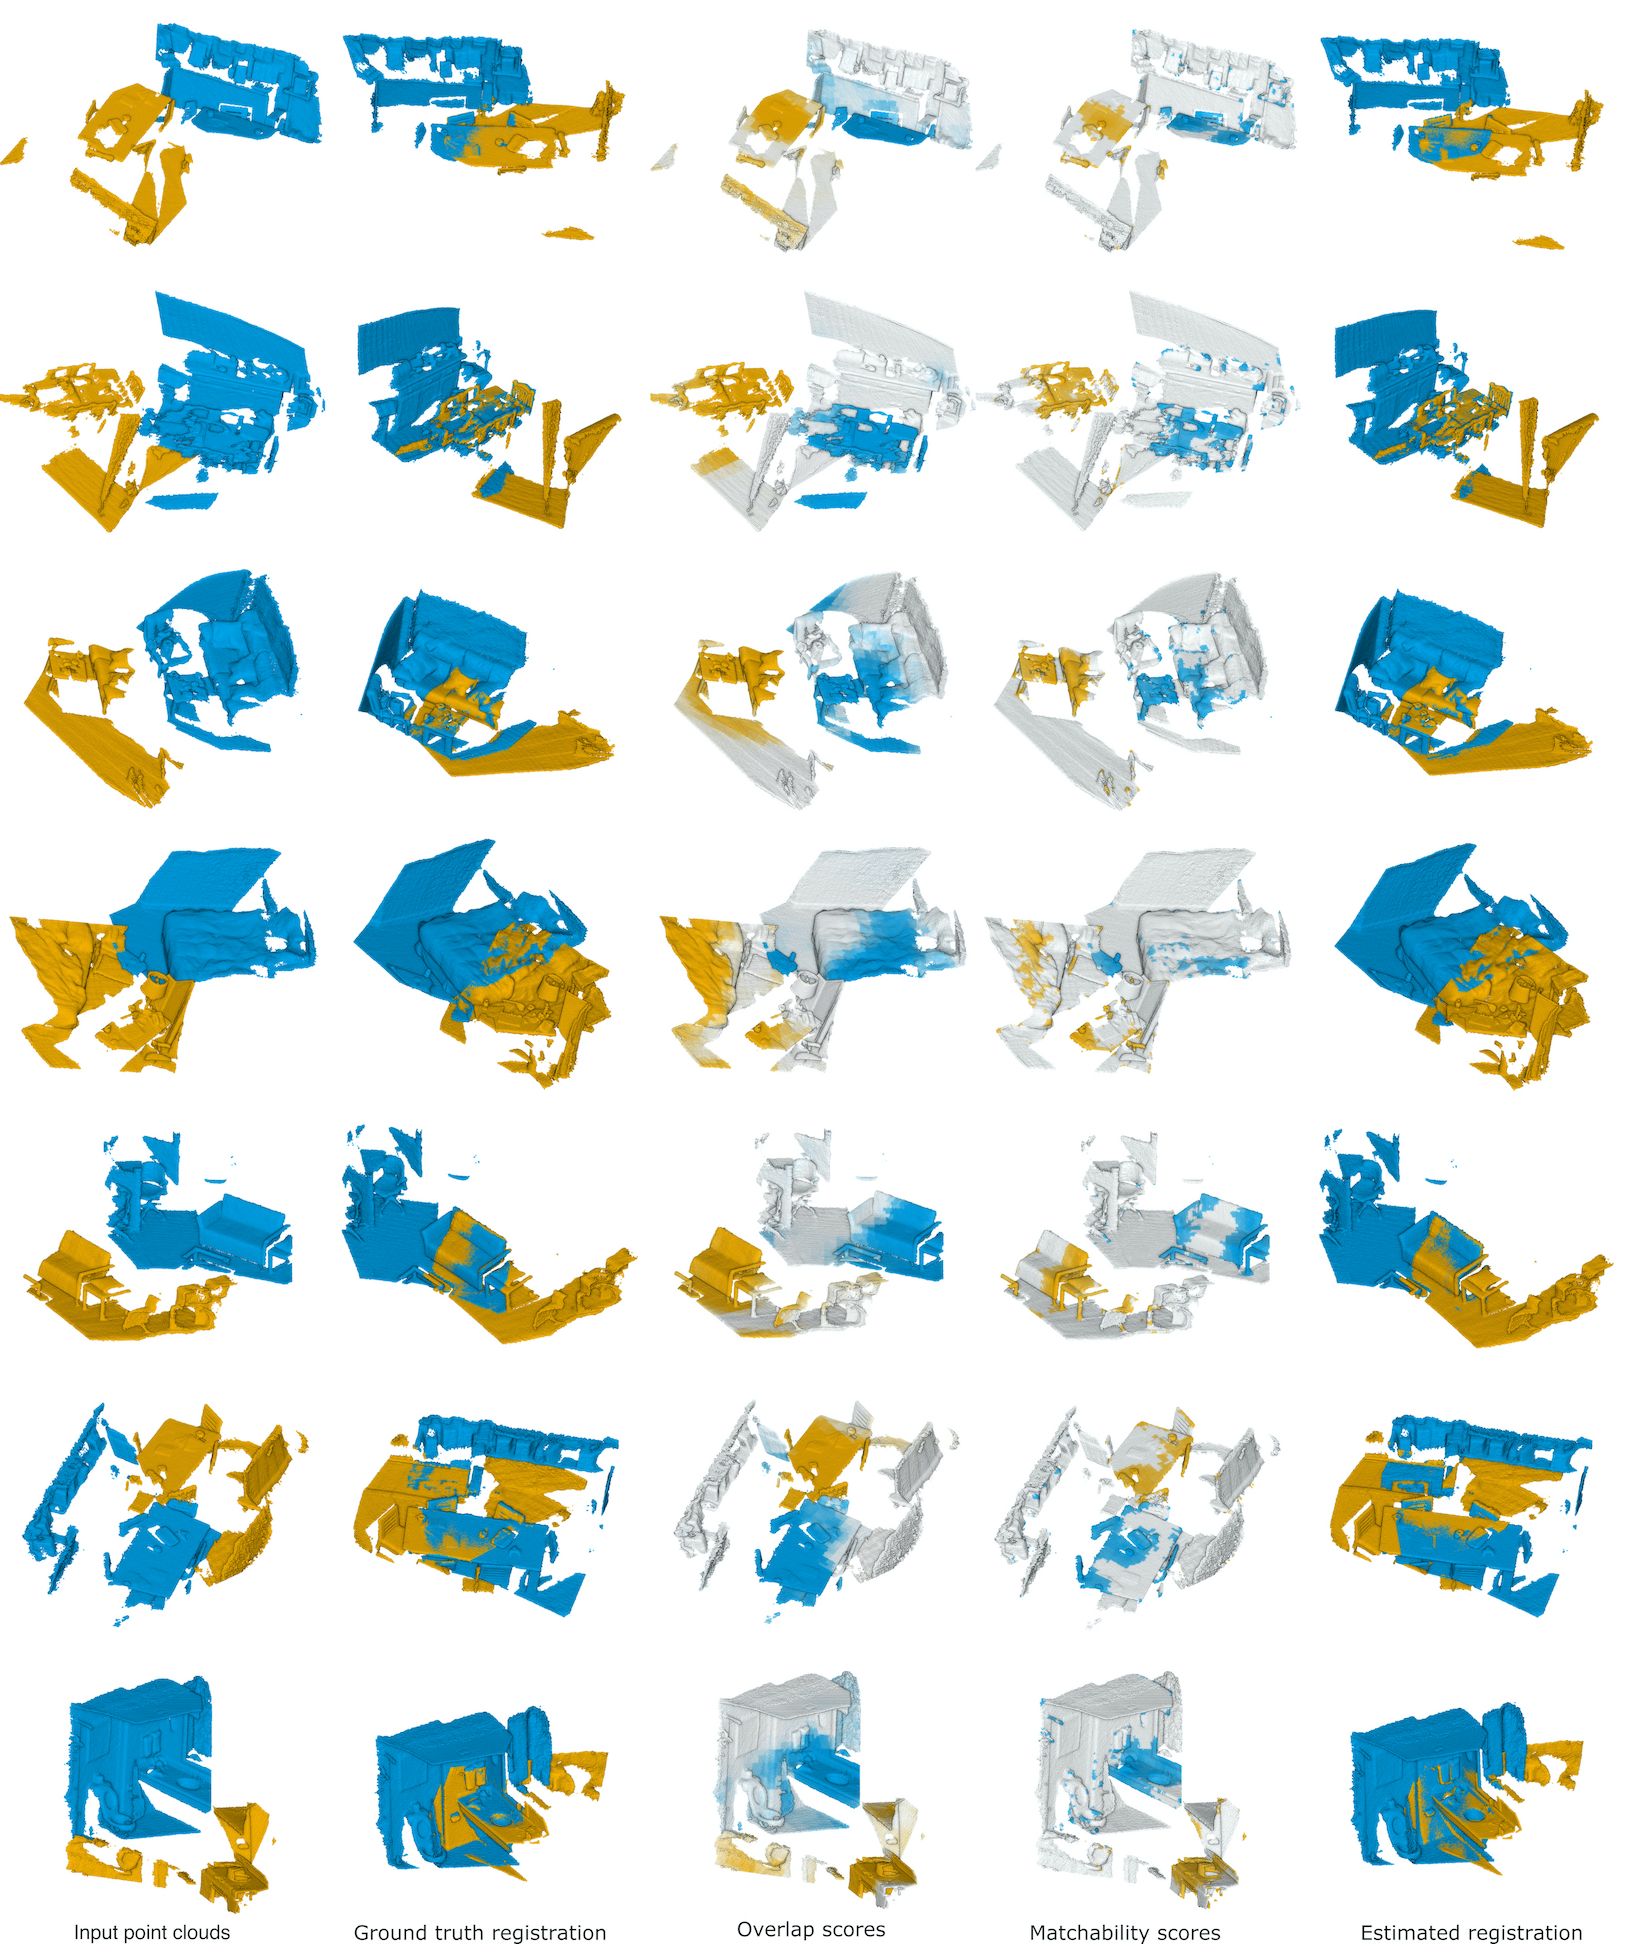
\includegraphics[width=\textwidth]{figures/images/3dmatch_supp.jpg}
    \caption{Example results on \emph{3DLoMatch}.}
    \label{fig:3dmatch_supp}
\end{figure}
\begin{figure}[t]
    \centering
    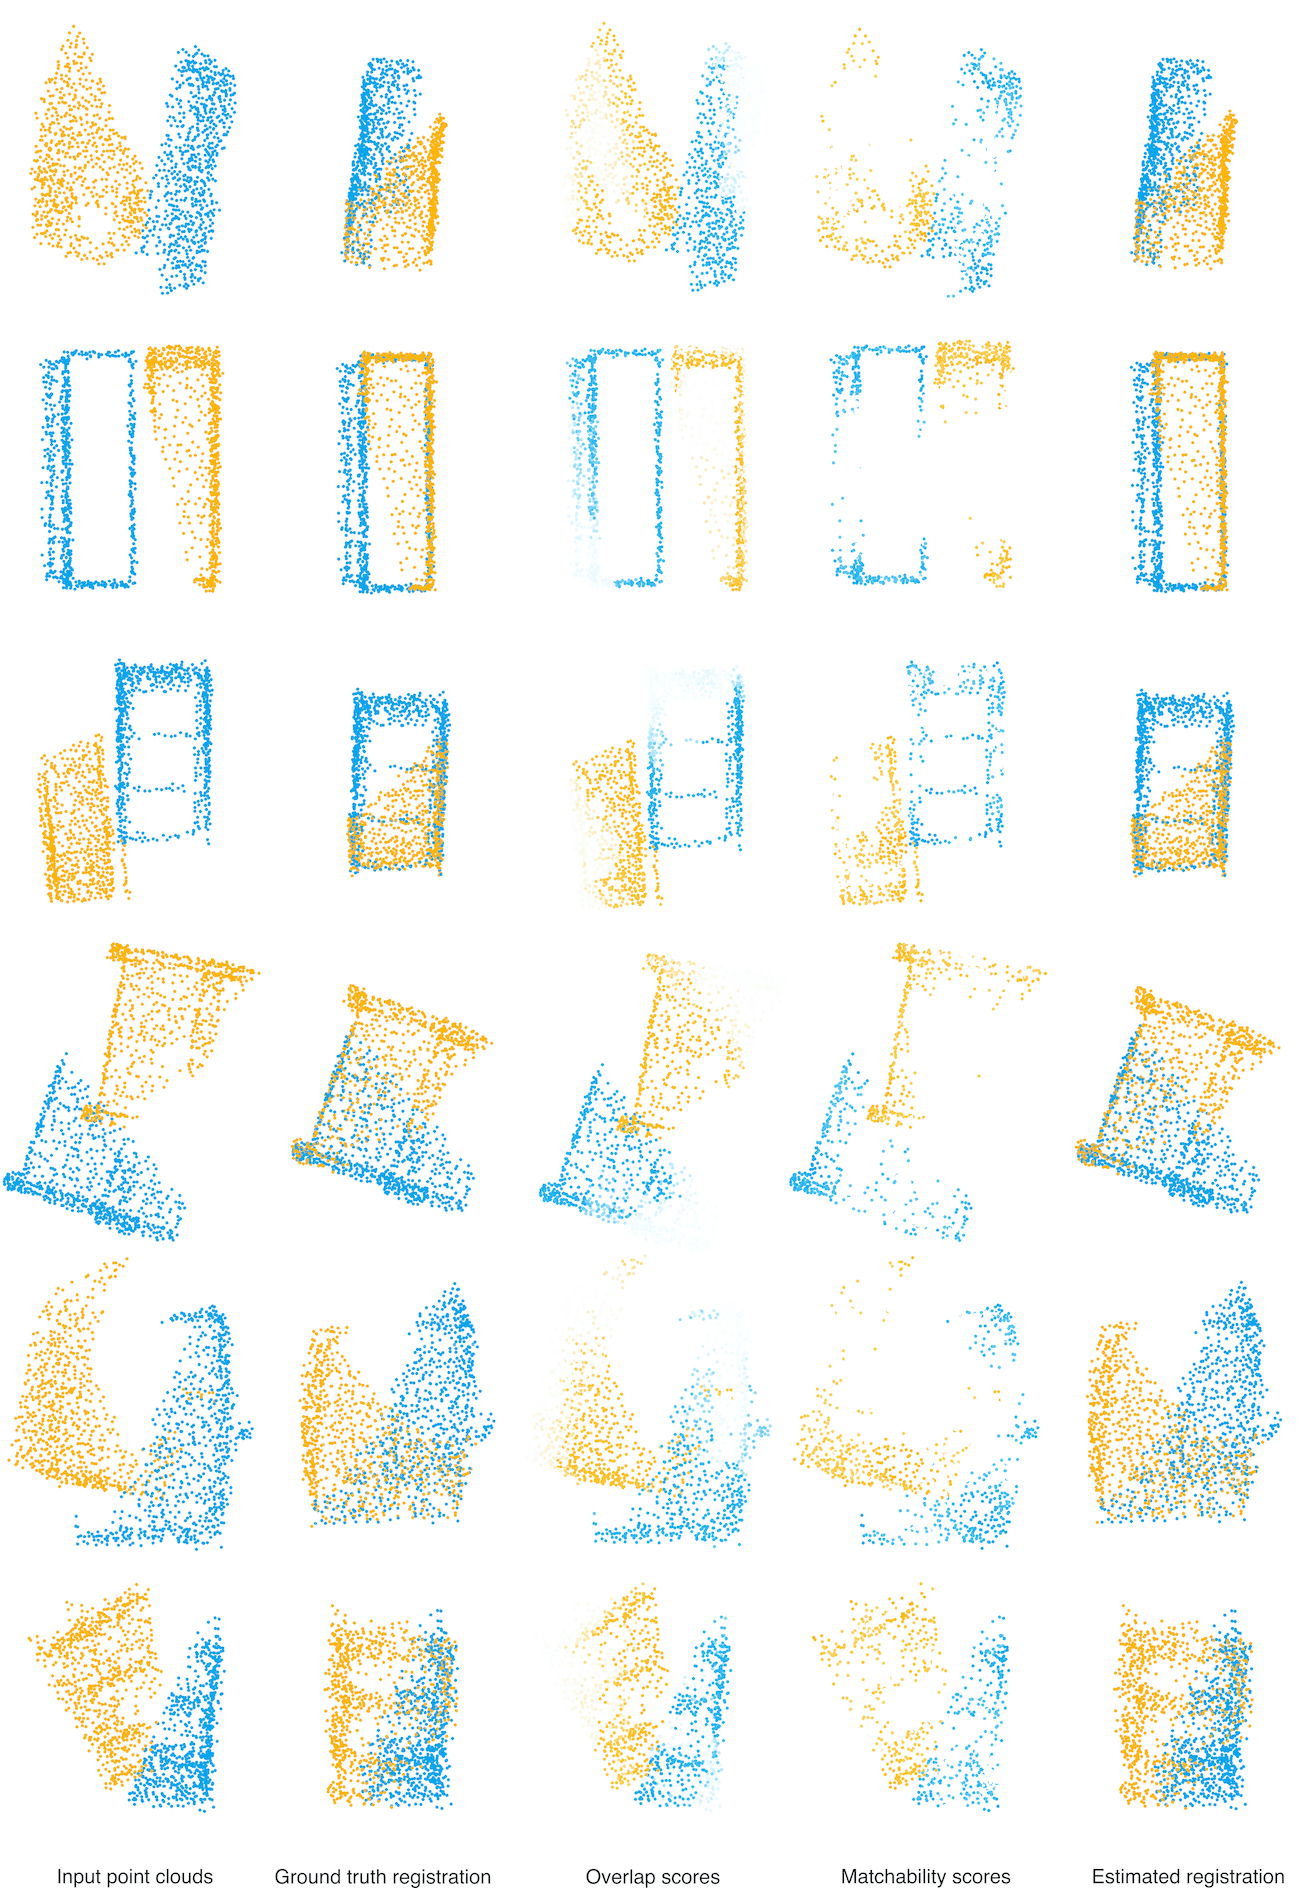
\includegraphics[width=0.87\columnwidth]{figures/images/modelnet_supp.jpg}
    \caption{Example results on \emph{ModelLoNet}.}
    \label{fig:modelnet_supp}
    
\end{figure}



